\documentclass{article}
\usepackage{float}
\usepackage{graphicx}
\begin{document}
	
	Sachin Ramesh Tendulkar (born 24th April 1973) is a former Indian international cricketer and a former captain of the Indian national team, regarded as one of the greatest batsman of all time. He is the highest run scorer of all time in International cricket. Tendulkar took up cricket at the age of eleven, made his Test debut on 15 November 1989 against Pakistan in Karachi at the age of sixteen, and went on to represent Mumbai domestically and India internationally for close to twenty-four years. He is the only player to have scored one hundred international centuries, the first batsman to score a double century in a ODI, the holder of the record for the most number of runs in both Test and ODI, and the only player to complete more than 30,000 runs in international cricket. He is colloquially known as Little Master or Master Blaster, and often referred to as the God of Cricket by Indian cricket followers. In 2001, Sachin Tendulkar became the first batsman to complete 10,000 ODI runs in his 259 innings. In 2002, halfway through his career, Wisden Cricketers' Almanack ranked him the second greatest Test batsman of all time, behind Don Bradman, and the second greatest ODI batsman of all time, behind Viv Richards.
	
	\hfill---author
	\ref{sachin}
	
	refer to table\ref{cs1}\\
	
	\begin{table}[h]
	\centering
	\begin{tabular}{|l|c|c|r|}
		\hline
		\textbf{Type}&\textbf{Matches}&\textbf{Runs}&\textbf{avg}\\
		\hline
		\hline
		test& 200 & 15361 & 56.01\\
		\hline
		ODI & 463 & 18561 & 44.83\\
		\hline
	\end{tabular}
	\caption{career statistics}
	\end{table}

	\begin{table}
	\centering
	\label{cs1}
	\begin{tabular}{|l|c|r|}
		\hline
		\textbf{Type}&\textbf{Matches}&\textbf{Runs}\\
		\hline
		\hline
		ODI & 463 & 18561\\
		\hline
	\end{tabular}
	\caption{career statistics}
	\end{table}

	\begin{figure}
		\centering
		\label{sachin}
		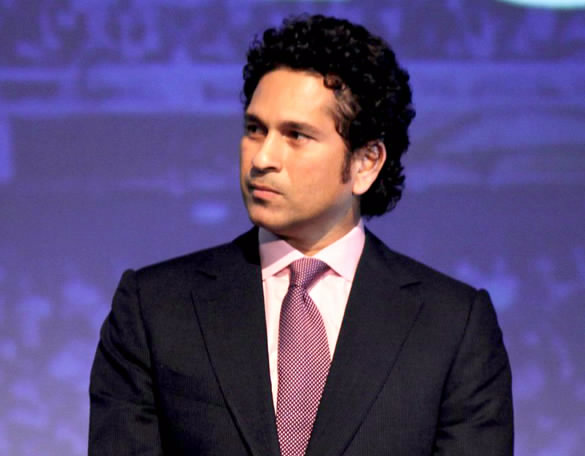
\includegraphics[scale = 0.25]{Sachin-01.jpg}
		\caption{figure1:Sachin}
	\end{figure}

	\pagebreak
	National awards and recieved are
	\begin{itemize}
		\item arjuna award
			\begin{enumerate}
				\item 1995
				\item 1996
			\end{enumerate}
		\item padma vibhooshan
		\item National award
		\item Bharatharatna
	\end{itemize}
	\pagebreak
	
	the general equation of quadratic eqution is $ax^{2}+bx+c$
	
	$ax_{1}+bx_{2}+cx_{3}$
	
	where $a$ is the coefficient of $x^{2}$, $b$ is the coefficient of x, c is the constant
	
	\begin{displaymath}
		ax^{2}+bx+c
	\end{displaymath}

	\begin{equation}
		ax^{2}+bx+c
	\end{equation}


	$\cos 2\theta = \cos^{2}\theta - \sin^{2}\theta$
	\begin{equation}
		\lim_{x\to\infty} \exp(-x) = 0
	\end{equation}
	$x\equiv a\pmod b$

		

\end{document}